\section{Data Acquisition, SITS Datasets and Preprocessing}

\begin{frame}{Data Sources: Varda Global FieldID}
\begin{block}{Parcel Geometries}
A collaborative database providing spatial delineations of agricultural plots worldwide.
\end{block}
%\pause
\begin{figure}
\centering
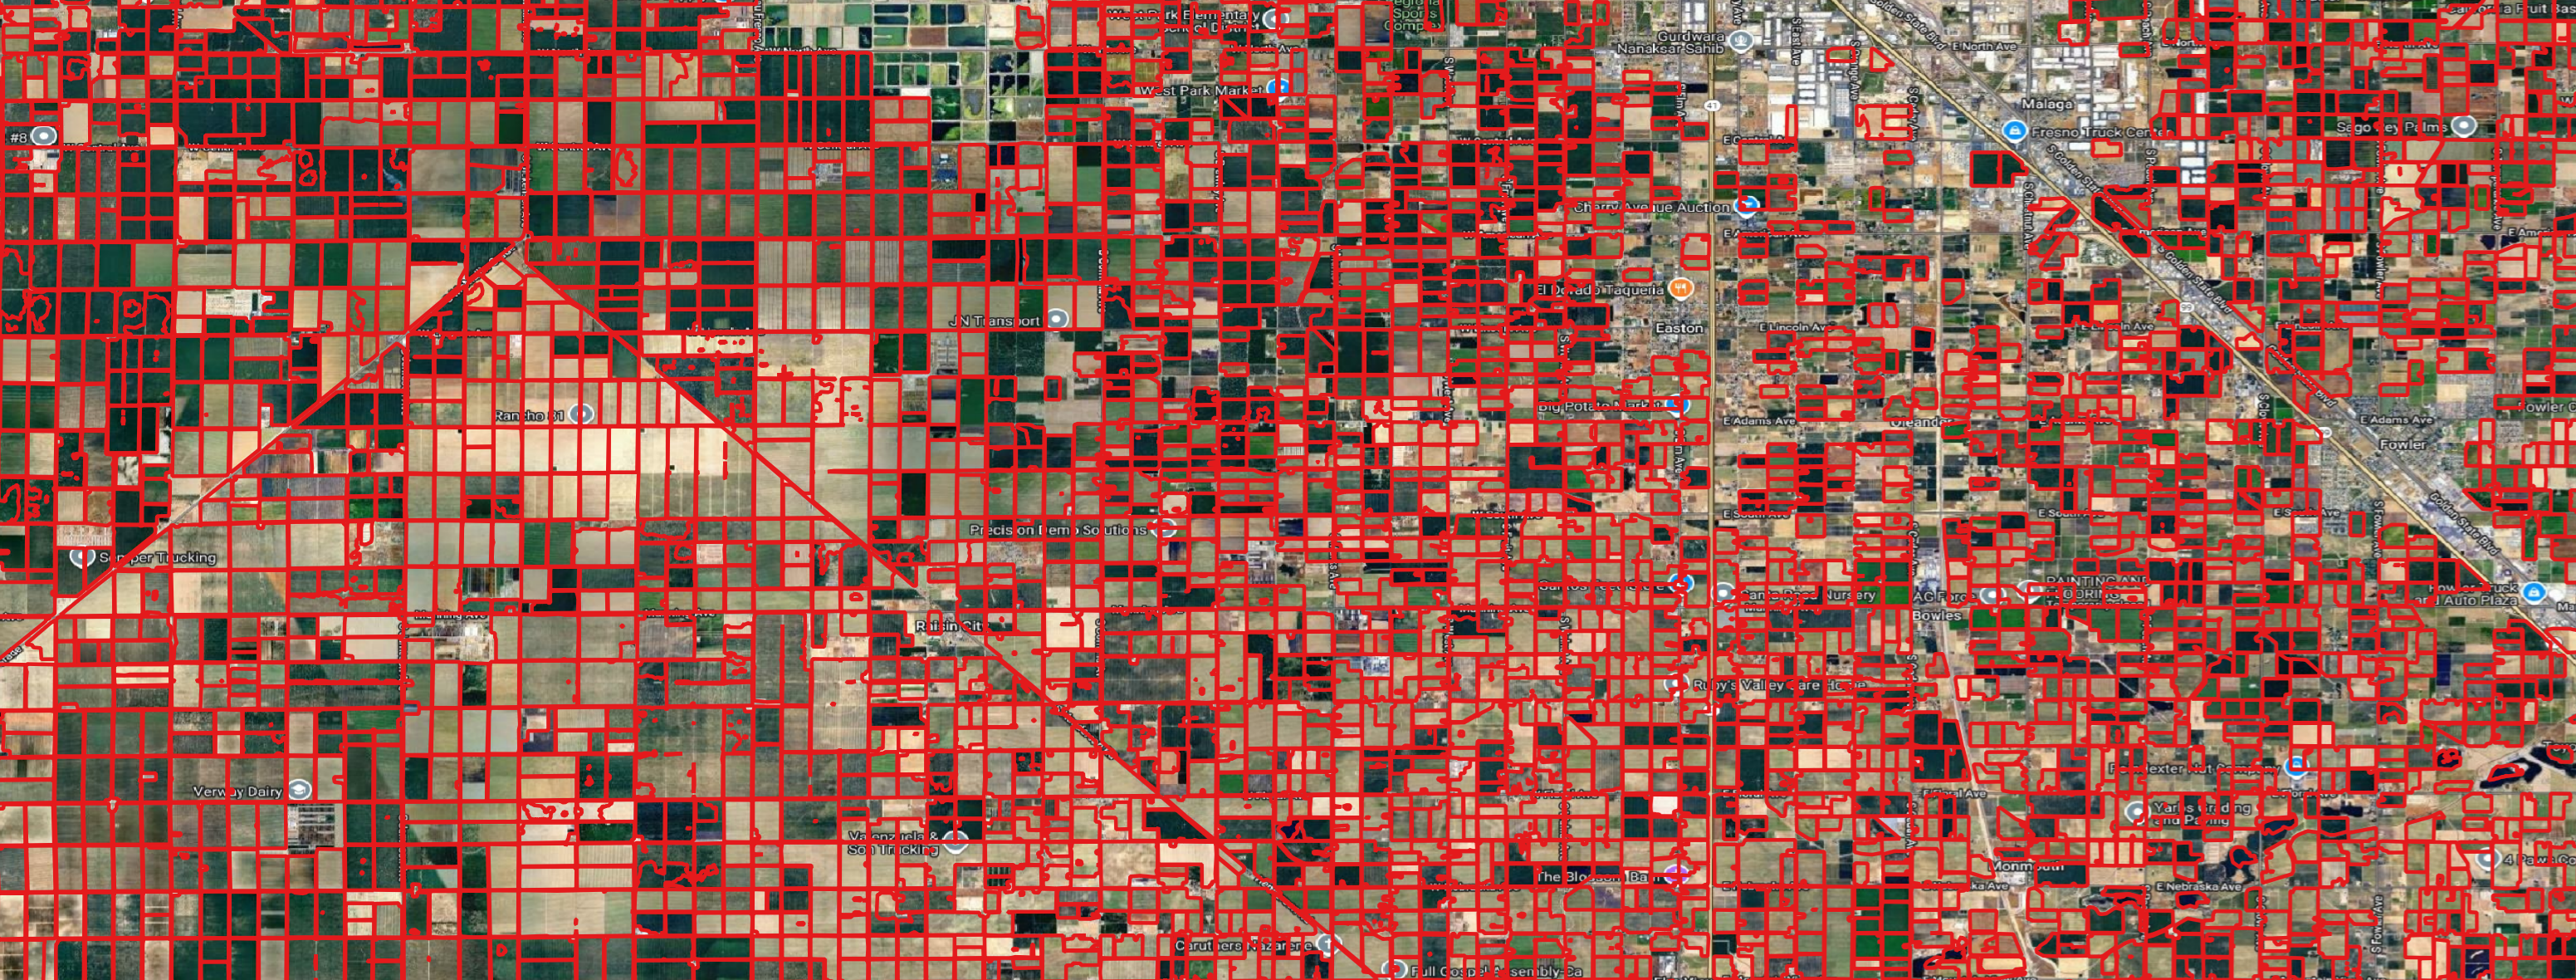
\includegraphics[width=\textwidth]{figures/6_methodology/varda/varda_fresno.png} 
\caption*{Well-delineated parcels in Fresno, California.}
\end{figure}
\end{frame}

\begin{frame}{Data Sources: Varda Global FieldID}
\renewcommand{\currprop}{1\textheight}
\begin{block}{The Challenge}
Public data contains noise, such as parcels mistakenly identified in water bodies, requiring strict filtering.
\end{block}
%\pause
\begin{figure}
\centering
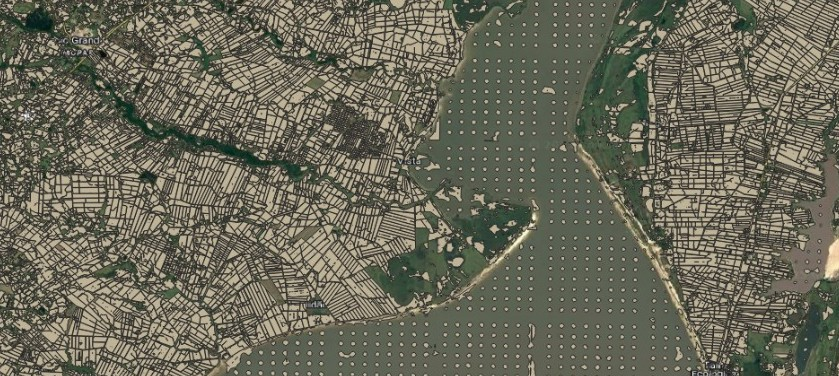
\includegraphics[width=0.9\textwidth]{figures_slides/varda_erros_slide.jpg}
\caption*{Mistakenly identified plots in water of Lagoa dos Patos.}
\end{figure}
\end{frame}

\begin{frame}{Data Sources: MapBiomas Brazil}
    \begin{columns}[c]
        \begin{column}{0.5\textwidth}
            \begin{block}{Brazilian Labels}
                Annual Land Use and Land Cover maps covering the historical series from 1985 to the present (30m resolution).
            \end{block}
            %\pause
            \begin{block}{Agricultural Theme}
                Subdivides into temporary and perennial crops (e.g., Soybean, Sugar Cane, Pasture, Coffee, Citrus).
            \end{block}
        \end{column}
        \begin{column}{0.5\textwidth}
            \begin{figure}
                \centering
                % Figura 40 da dissertação
                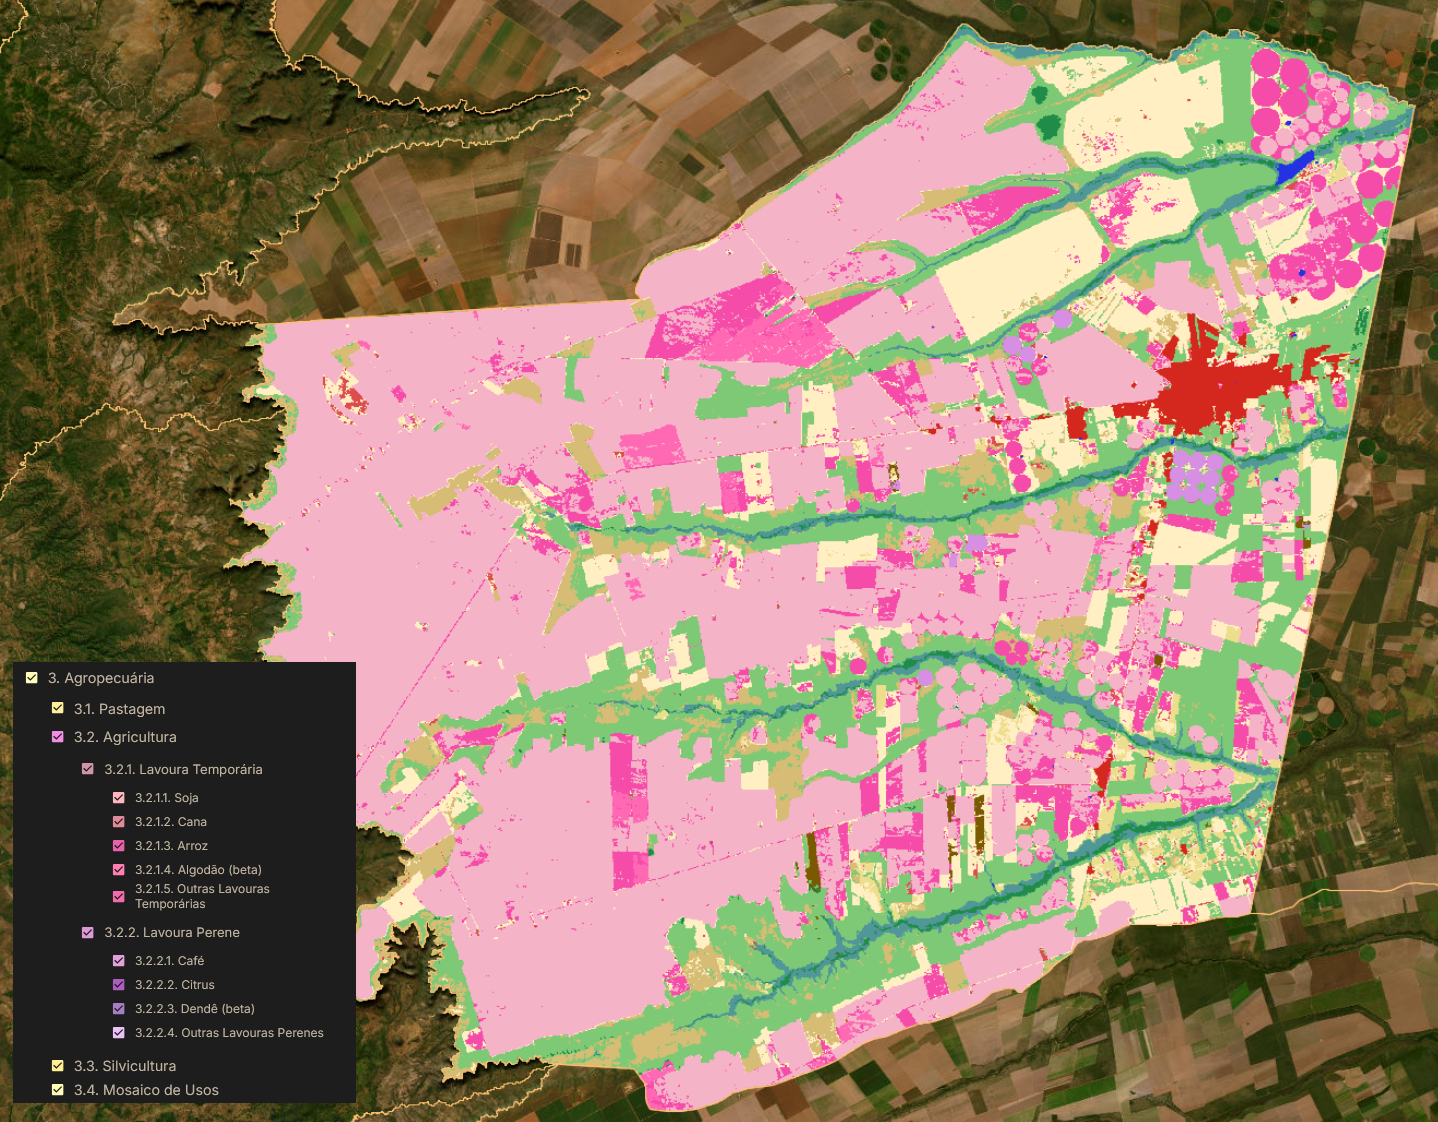
\includegraphics[width=0.9\textwidth]{figures/6_methodology/mapbiomas.png} 
                \caption*{MapBiomas Cropland Raster}
            \end{figure}
        \end{column}
    \end{columns}
\end{frame}

\begin{frame}{Data Sources: USDA Cropland Data Layer (CDL)}
    \begin{columns}[c]
        \begin{column}{0.5\textwidth}
            \begin{block}{USA Labels}
                High-resolution specific agricultural crop masks provided by the National Agricultural Statistics Service (NASS).
            \end{block}
            %\pause
            \begin{block}{Coverage}
                Used to extract specific crop labels for the Texas and California datasets (e.g., Corn, Cotton, Almonds).
            \end{block}
        \end{column}
        \begin{column}{0.5\textwidth}
            \begin{figure}
                \centering
                % Figura 41 da dissertação
                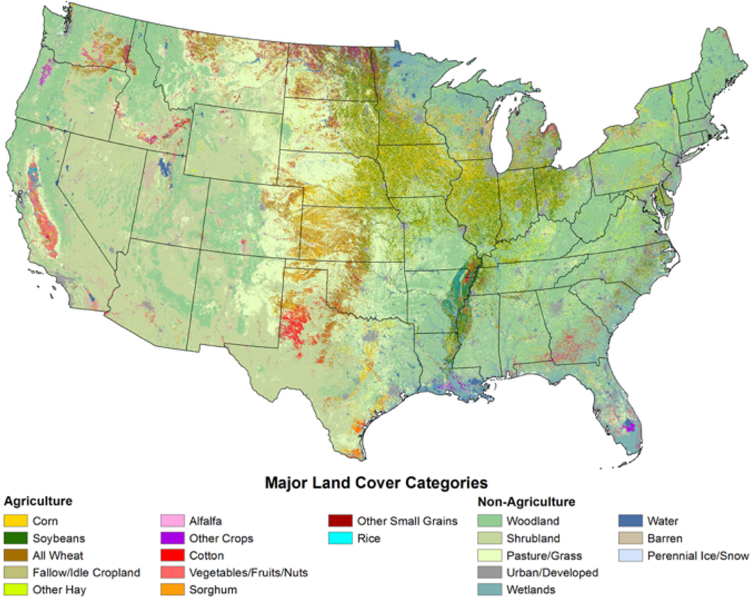
\includegraphics[width=0.9\textwidth]{figures/6_methodology/USDA.png} 
                \caption*{USDA CDL Raster}
            \end{figure}
        \end{column}
    \end{columns}
\end{frame}


\begin{frame}{Lightweight SITS Download Strategy}
    \renewcommand{\currprop}{0.6\textheight}
    
    \begin{block}{Acquiring high confidence labels and features}
    \only<1| handout:0>{We initiate the pipeline by matching raw cropland rasters with precise parcel delineations}%
    \only<2| handout:0>{This data is processed within GEE Cloud (using our library) to extract comprehensive vegetation indices.}%
    \only<3| handout:0>{A vegetative filter basead on thresholds ensures the acquisition of highly reliable, high-confidence crop labels.}%
    \only<4| handout:0>{The result are high confidence parcel crop classification labels.}%
    \only<5| handout:0>{To explain the SITS download, let's take a look at a single sample.}%
    \only<6| handout:0>{Raw satellite images are selected if they intersect with the parcel geometry.}%
    \only<7| handout:0>{All images are cropped by the parcel geometry.}%
    \only<8| handout:0>{Clouds and cloud shadows pixels are filtered out in each image.}%
    \only<9| handout:0>{The clear pixels are then spatially aggregated to generate clear statistical metrics, such median.}%
    \only<10| handout:1>{The final result of the download strategy are treated resulting SITS and crop classes.}%
\end{block}
\begin{figure}
    \centering
    \includegraphics<1| handout:0>[height=\currprop]{figures_slides/datasets_8.jpg}%
    \includegraphics<2| handout:0>[height=\currprop]{figures_slides/datasets_7.jpg}%
    \includegraphics<3| handout:0>[height=\currprop]{figures_slides/datasets_6.jpg}%
    \includegraphics<4| handout:0>[height=\currprop]{figures_slides/datasets_5.jpg}%
    \includegraphics<5| handout:0>[height=\currprop]{figures_slides/datasets_4.jpg}%
    \includegraphics<6| handout:0>[height=\currprop]{figures_slides/datasets_3.jpg}%
    \includegraphics<7| handout:0>[height=\currprop]{figures_slides/datasets_2.jpg}%
    \includegraphics<8| handout:0>[height=\currprop]{figures_slides/datasets_1.jpg}%
    \includegraphics<9| handout:0>[height=\currprop]{figures_slides/datasets_0.jpg}%
    \includegraphics<10| handout:1>[height=\currprop]{figures_slides/datasets_final.jpg}%
\end{figure}
\end{frame}
\begin{frame}{The Proposed SITS Datasets}
    \begin{block}{Three Novel Parcel-Level Datasets}
        We generated three datasets: \textbf{Texas} (7 classes), \textbf{California} (14 classes), and \textbf{Brazil} (10 classes).
    \end{block}
    \pause
    \begin{block}{The Complexity of the Brazilian Dataset}
        Unlike the US regions (mostly single-cycle monocultures), Brazil presents unique challenges:
        \begin{itemize}
            \item \textbf{Subcontinental scale:} High regional variability in planting schedules across different biomes.
            \item \textbf{Double/Triple Cropping ("Safrinha"):} The presence of secondary crops acts as spectral noise, since public maps (like MapBiomas) provide only the primary crop label.
            \item \textbf{Noise from crop source:} MapBiomas deals with land use and cover, not active agriculture. 
        \end{itemize}
    \end{block}
\end{frame}

%%%%%%%%%%%%%%%%%%%%%%%%%%%%%%%%%%%%%%%%%%%%%%%%%%%%%%%%%%%%%%%%%%%%%%%%%%

\begin{frame}{Dataset Characteristics: Class Imbalance}
    \vspace{0.2cm}
    
    \begin{columns}[c]
        \begin{column}{0.33\textwidth}
            \begin{figure}
                \centering
                % Figura 44 da dissertação
                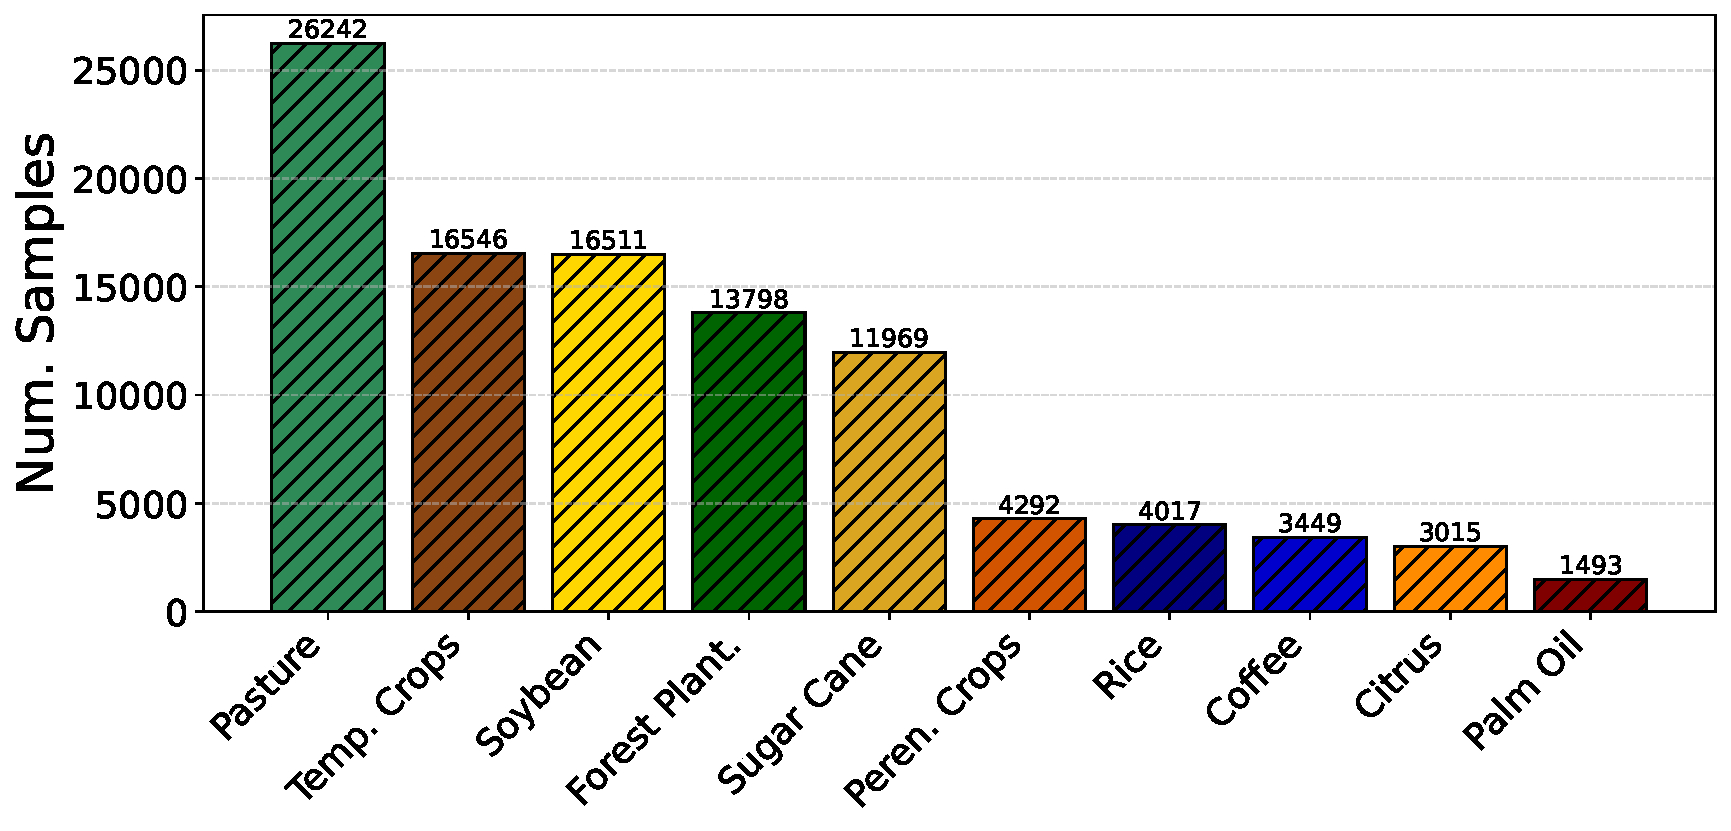
\includegraphics[width=\textwidth]{figures/6_methodology/datasets/brazil_bar_crop.pdf} 
                \caption*{Brazil (10 classes)}
            \end{figure}
        \end{column}
        \begin{column}{0.33\textwidth}
            \begin{figure}
                \centering
                % Figura 45 da dissertação
                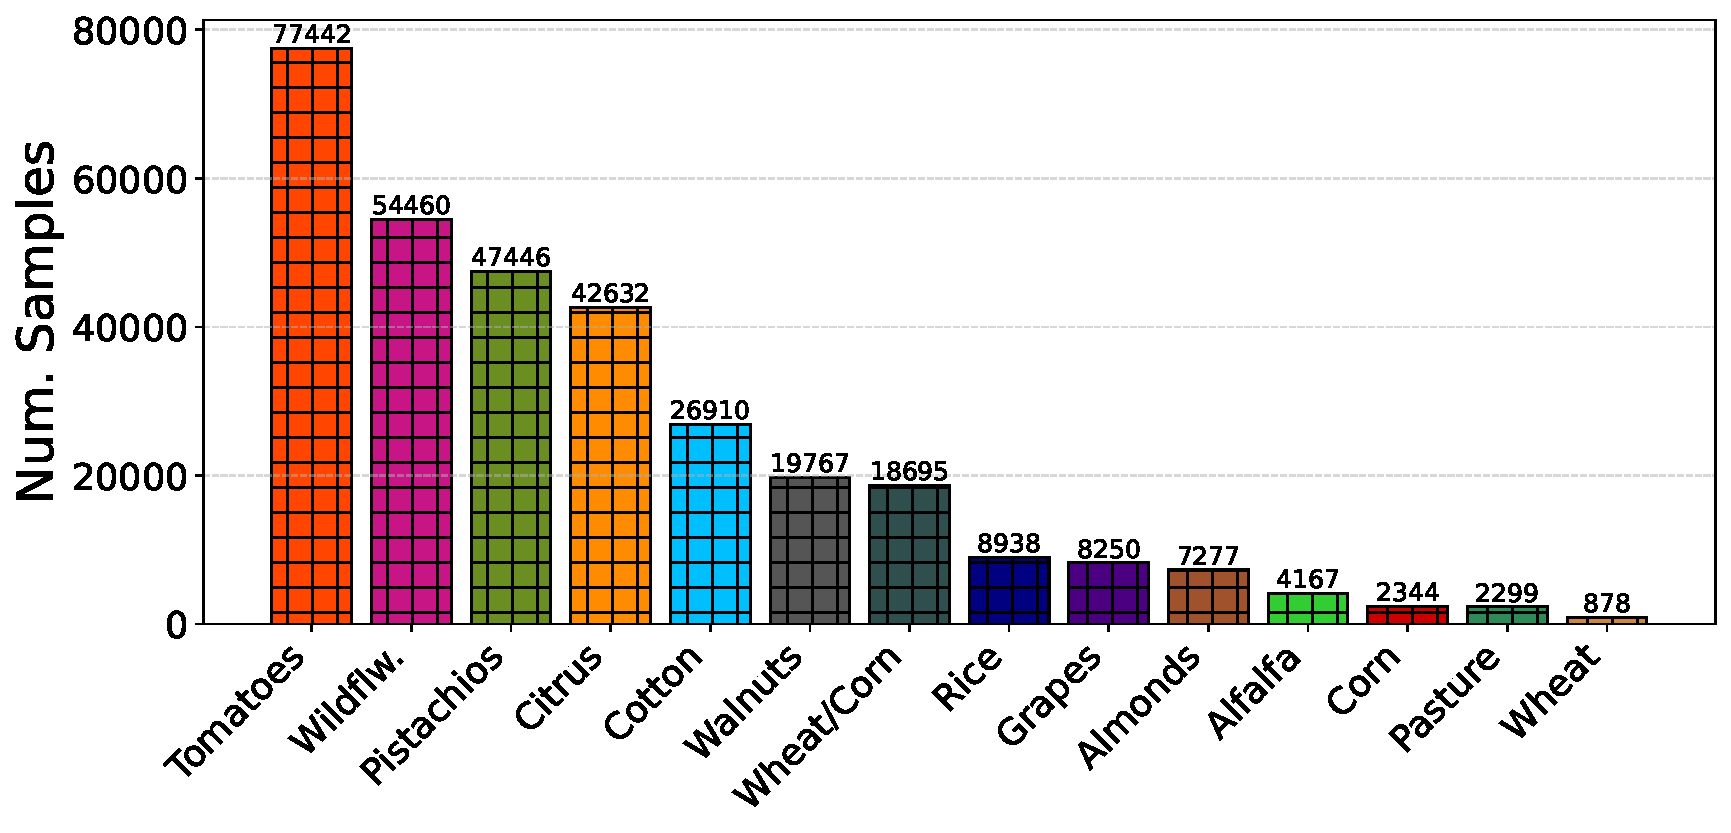
\includegraphics[width=\textwidth]{figures/6_methodology/datasets/california_bar_crop.pdf} 
                \caption*{California (14 classes)}
            \end{figure}
        \end{column}
        \begin{column}{0.33\textwidth}
            \begin{figure}
                \centering
                % Figura 46 da dissertação
                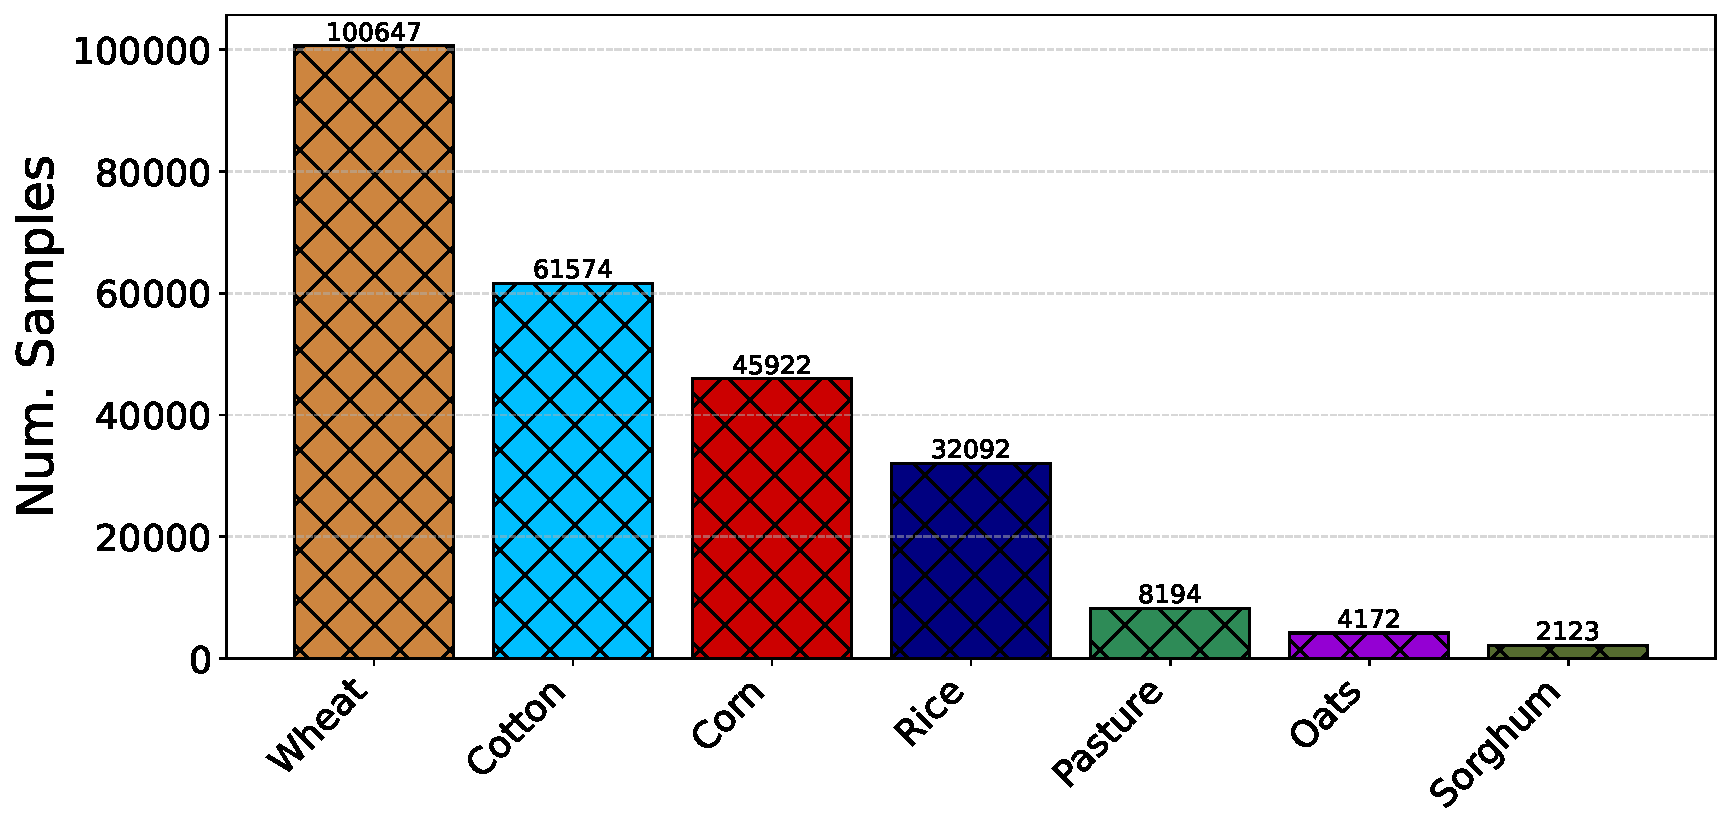
\includegraphics[width=\textwidth]{figures/6_methodology/datasets/texas_bar_crop.pdf} 
                \caption*{Texas (7 classes)}
            \end{figure}
        \end{column}
    \end{columns}
\end{frame}

\begin{frame}{Brazil Dataset Geospatial Distribution}
    \begin{figure}
        \centering
        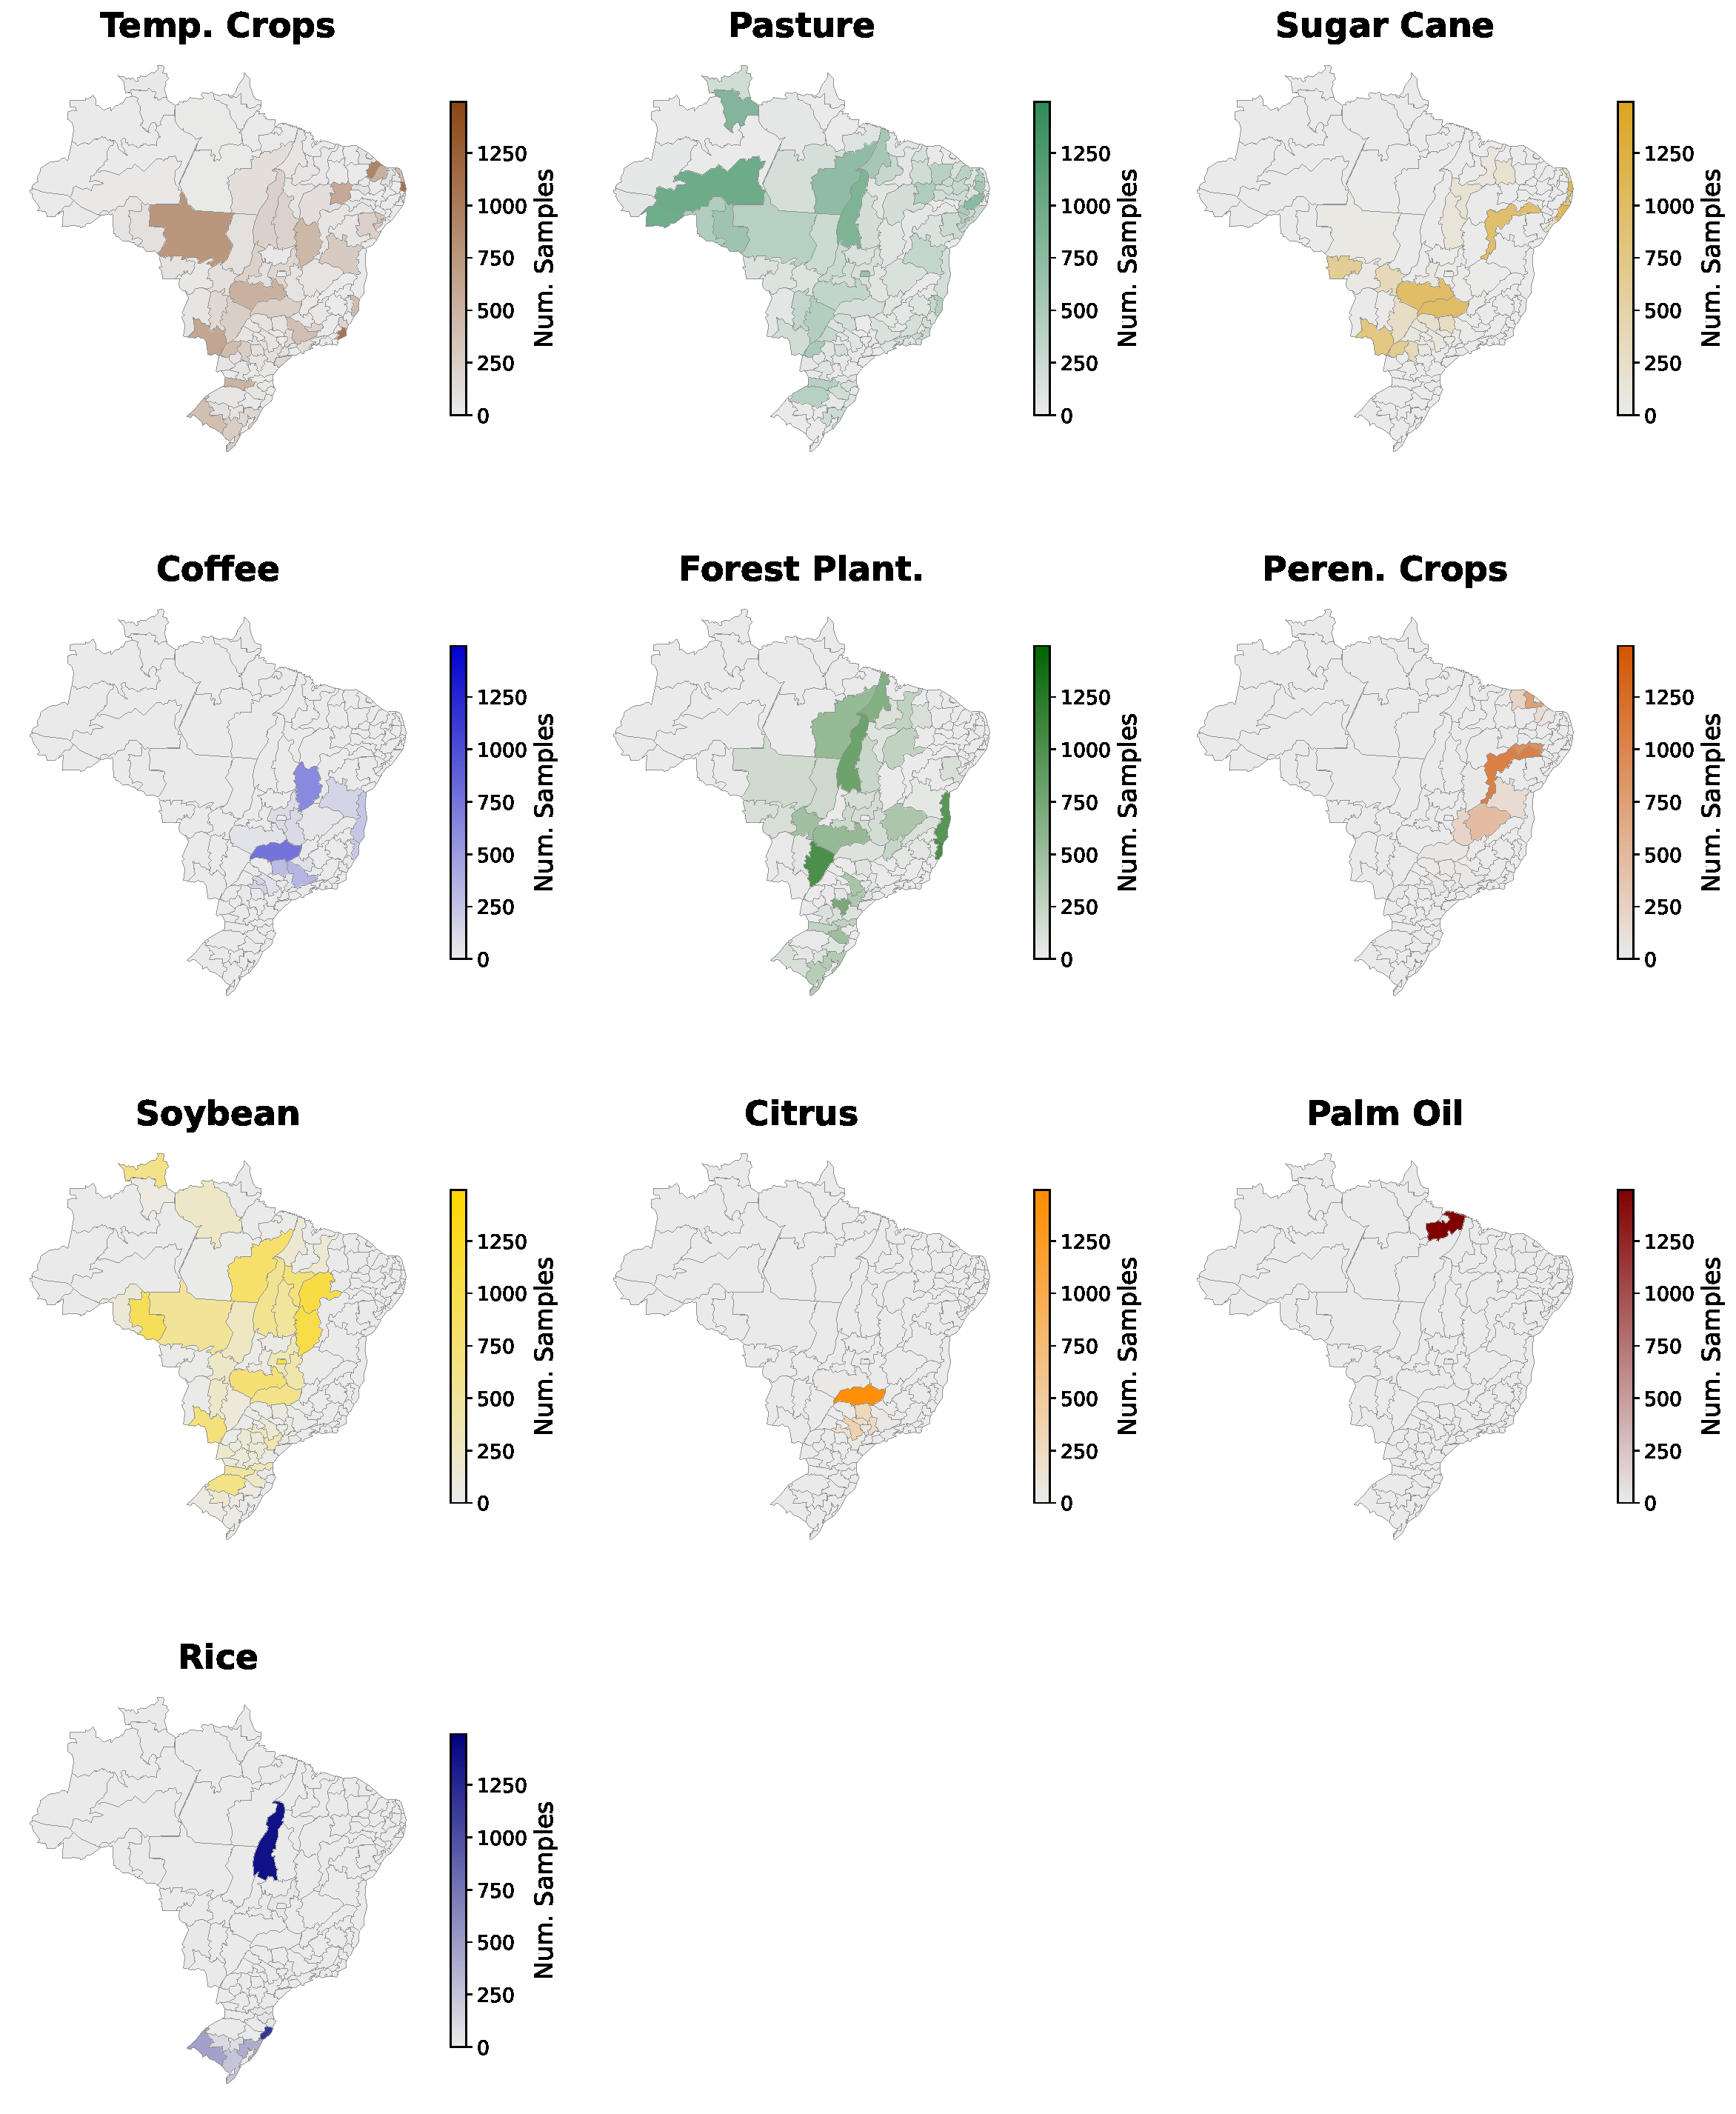
\includegraphics[width=0.7\textwidth]{figures/6_methodology/datasets/brazil_map_crops.pdf}
    \end{figure}
\end{frame}

% --- EVI2 SIGNATURES ---

\begin{frame}{Phenological Signatures (EVI2): Brazil Dataset}
    \begin{block}{The ``Safrinha'' Challenge}
        \begin{itemize}
            \item \textbf{Double Cropping \& Label Noise:} Temporary crops (e.g., Soybean) show secondary peaks. MapBiomas maps only the primary crop, adding spectral noise.
            \item \textbf{Perennials:} Classes like Forest Plantation exhibit stable, high EVI2 values year-round.
        \end{itemize}
    \end{block}
    
    \begin{figure}
        \centering
        % Figura 48 da dissertação
        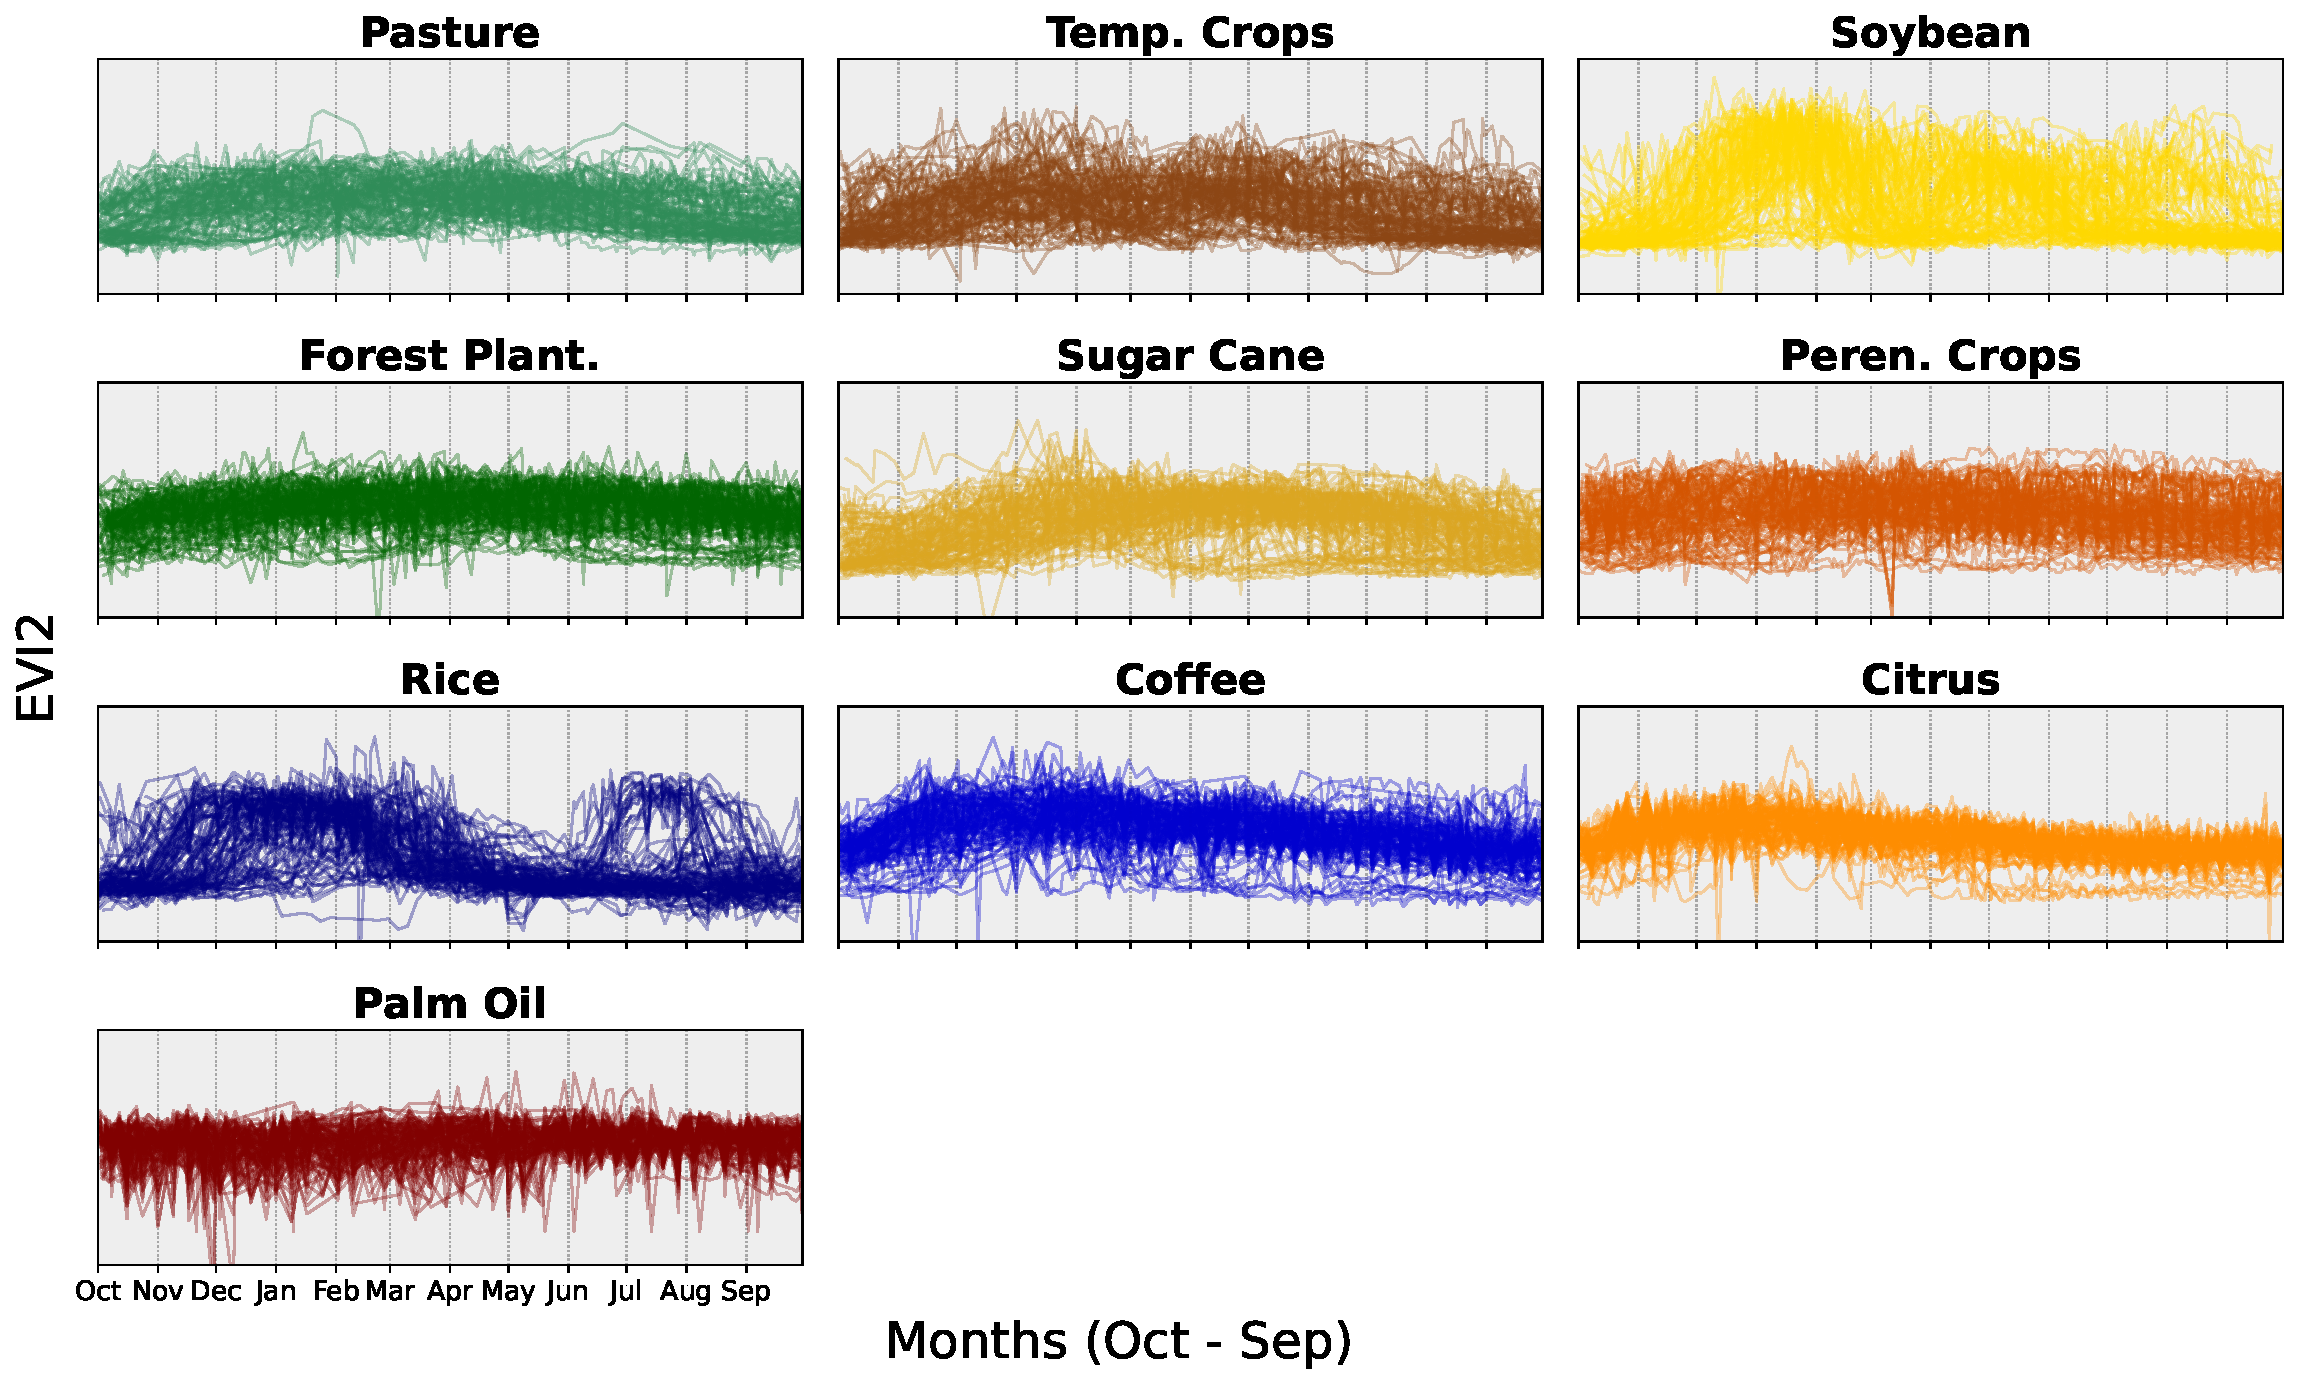
\includegraphics[height=0.4\textheight, width=\textwidth, keepaspectratio]{figures/6_methodology/datasets/brazil_evi2.pdf} 
    \end{figure}
\end{frame}

\begin{frame}{Phenological Signatures (EVI2): California Dataset}
    \begin{block}{Crop Signatures in California}
        \begin{itemize}
            \item \textbf{Clearer Signatures:} More pronounced behaviors and less label noise than Brazil.
            \item \textbf{Single-cycle:} Predominantly single-cycle crops.
            \item \textbf{Rotation:} A specific labeled class (\textit{Wheat/Corn}) exhibits a distinct double-peak signature.
        \end{itemize}
    \end{block}
    
    \begin{figure}
        \centering
        % Figura 49 da dissertação
        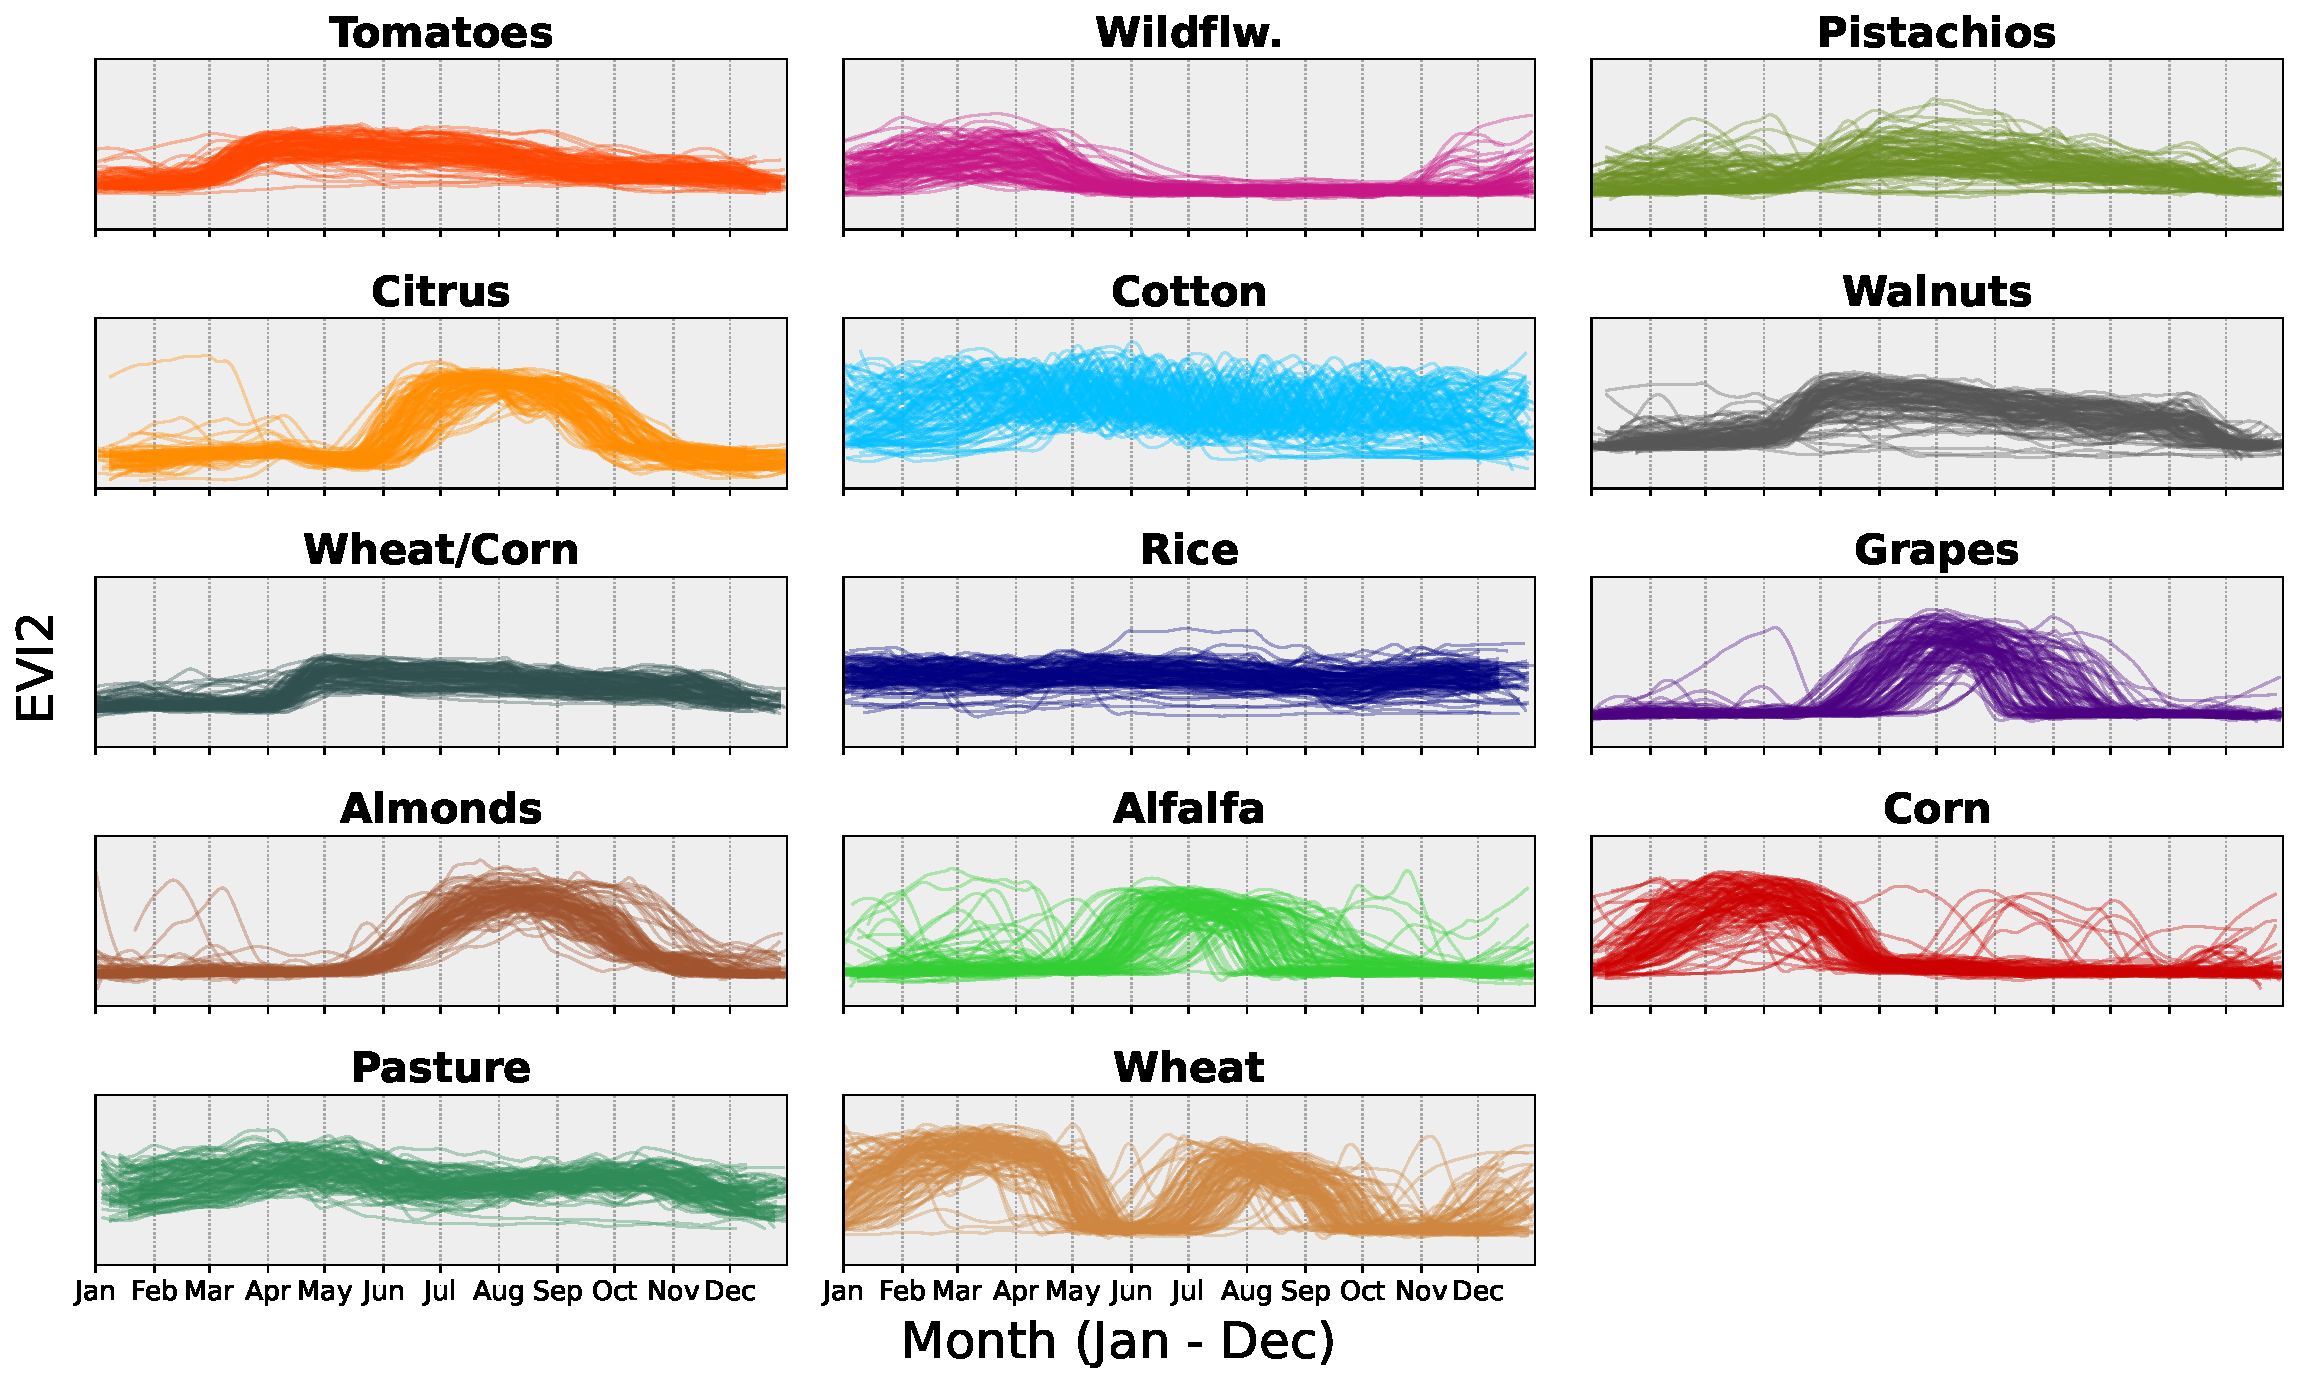
\includegraphics[height=0.4\textheight, width=\textwidth, keepaspectratio]{figures/6_methodology/datasets/california_evi2.pdf} 
    \end{figure}
\end{frame}

\begin{frame}{Phenological Signatures (EVI2): Texas Dataset}
    \begin{block}{Crop Signatures in Texas}
        \begin{itemize}
            \item \textbf{Clearest Separation:} The clearest spectral separation among all regions evaluated.
            \item \textbf{Monocultures:} Dominated by single-cycle crops with clear, single-peak curves (e.g., Cotton, Corn).
            \item \textbf{Fallow Periods:} Long, well-defined fallow periods ease the classification task.
        \end{itemize}
    \end{block}
    
    \begin{figure}
        \centering
        % Figura 50 da dissertação
        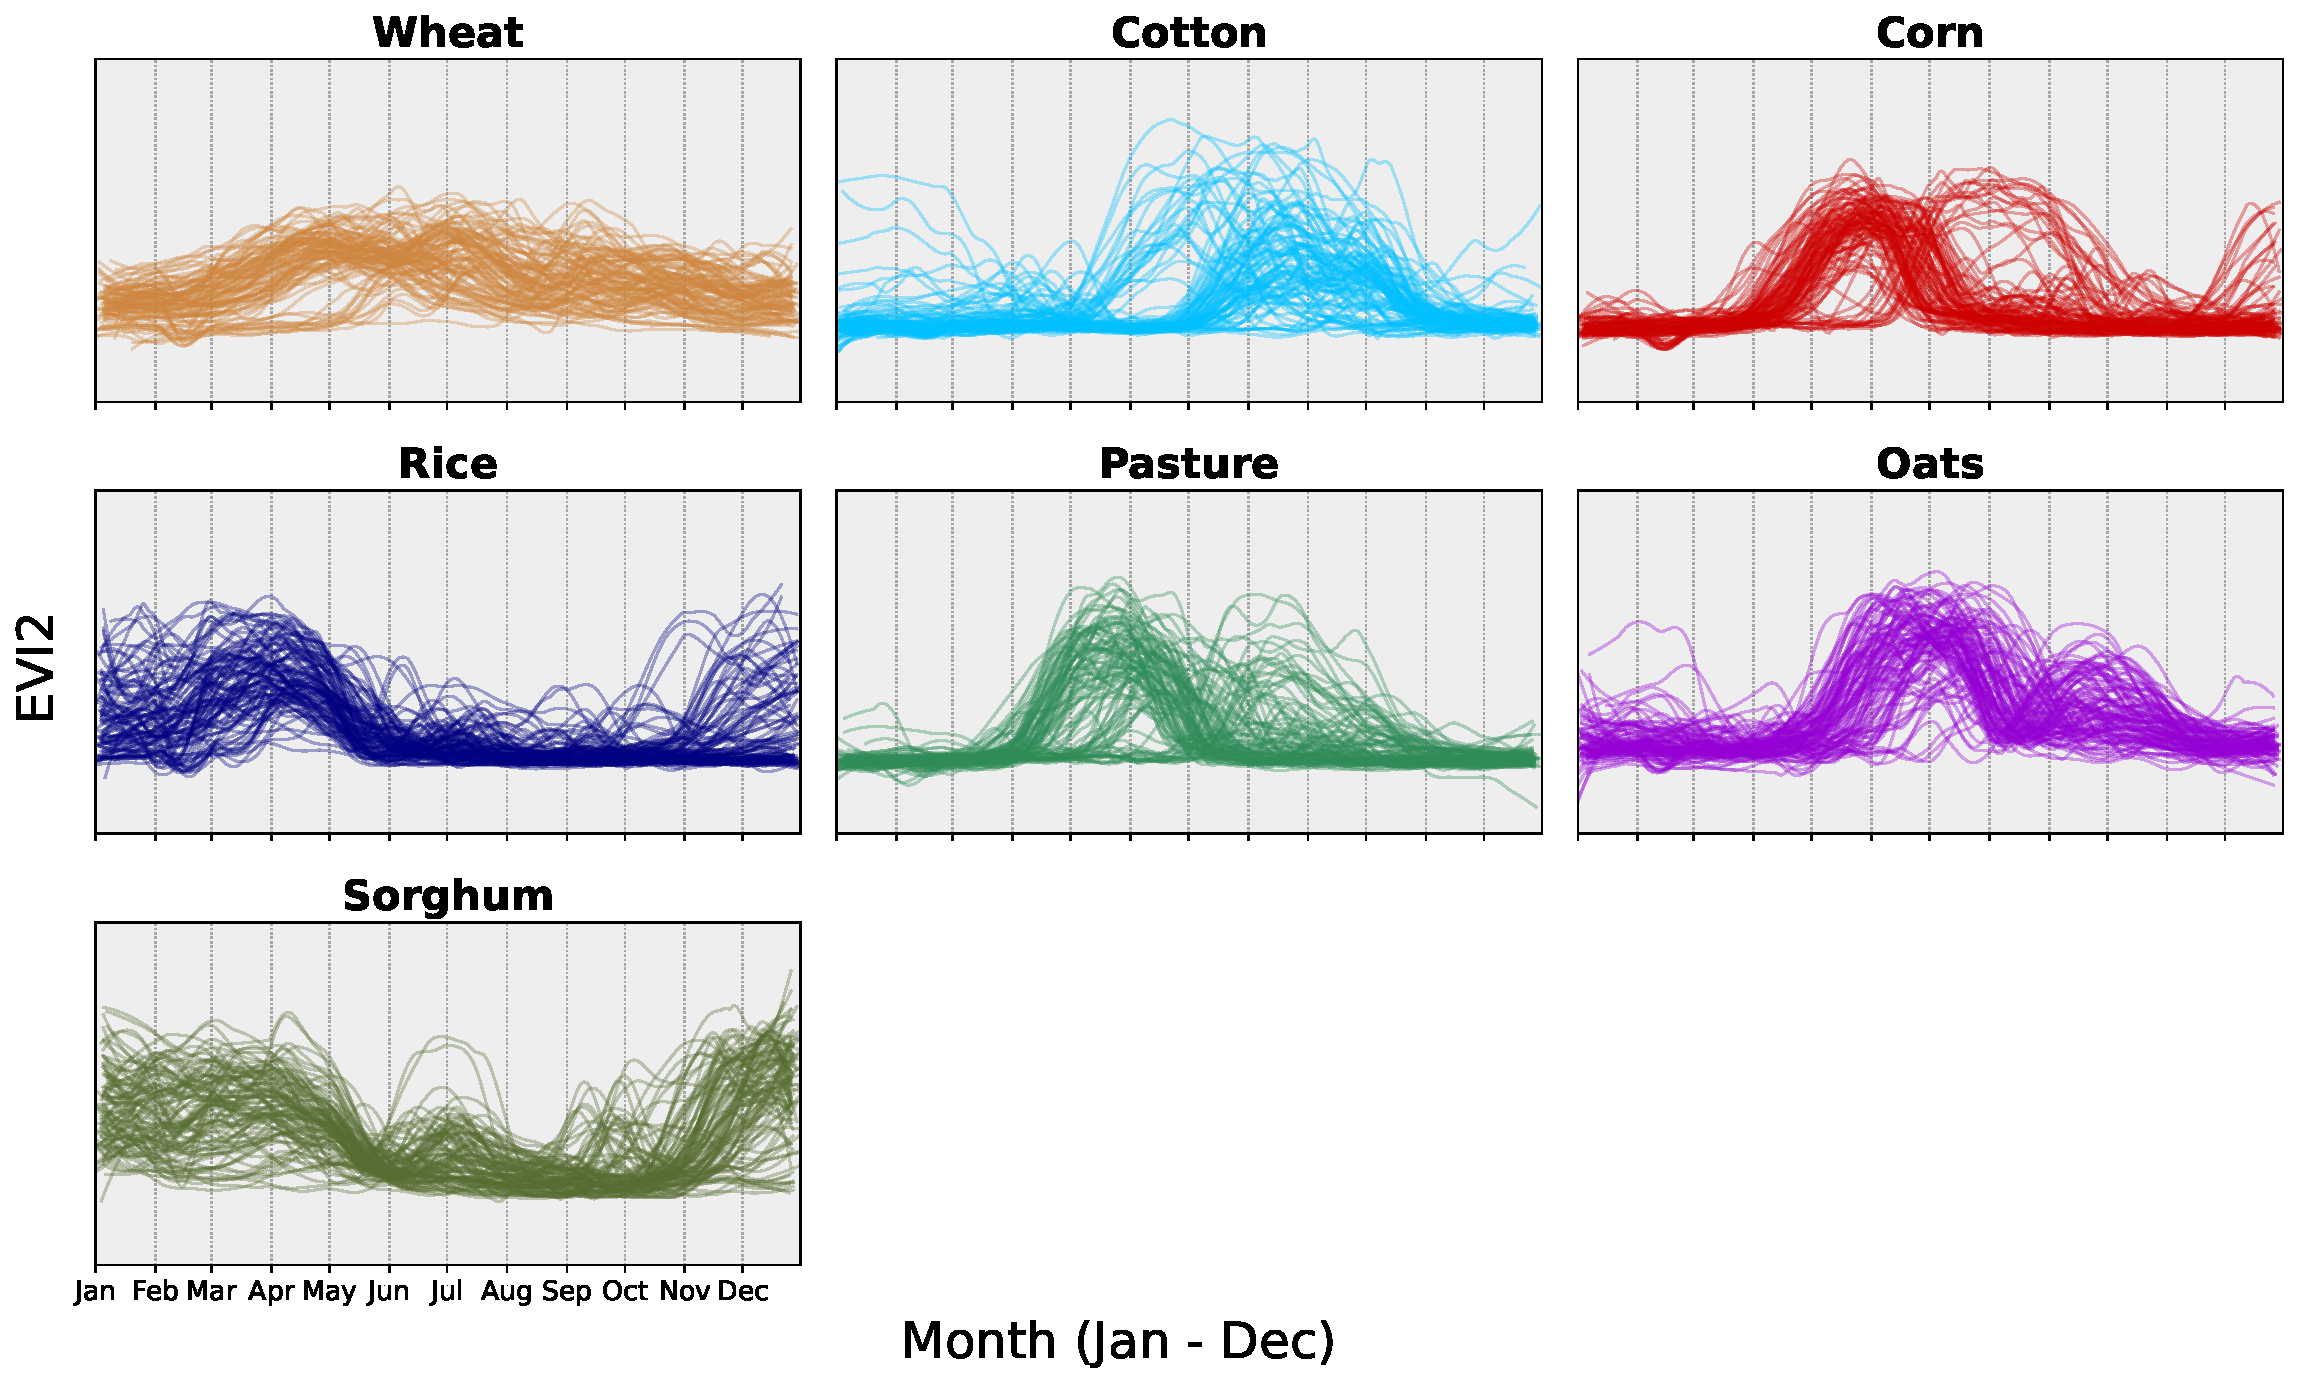
\includegraphics[height=0.4\textheight, width=\textwidth, keepaspectratio]{figures/6_methodology/datasets/texas_evi2.pdf} 
    \end{figure}
\end{frame}